\chapter{Глибина зразка (Sample depth)}\label{cha:sample_depth}
Значення пікселів потрібно зберігати в пам’яті комп’ютерів, це означає, що врешті-решт дані повинні в кінцевому підсумку потрапити у двійкове представлення, просторова безперервність зображення апроксимується інтервалом вибірки в сітці зразків.

Значення, які ми можемо представити для кожного пікселя, визначаються обраним зразком формату.

\begin{figure}
    \label{fig:image6}
    \centering
    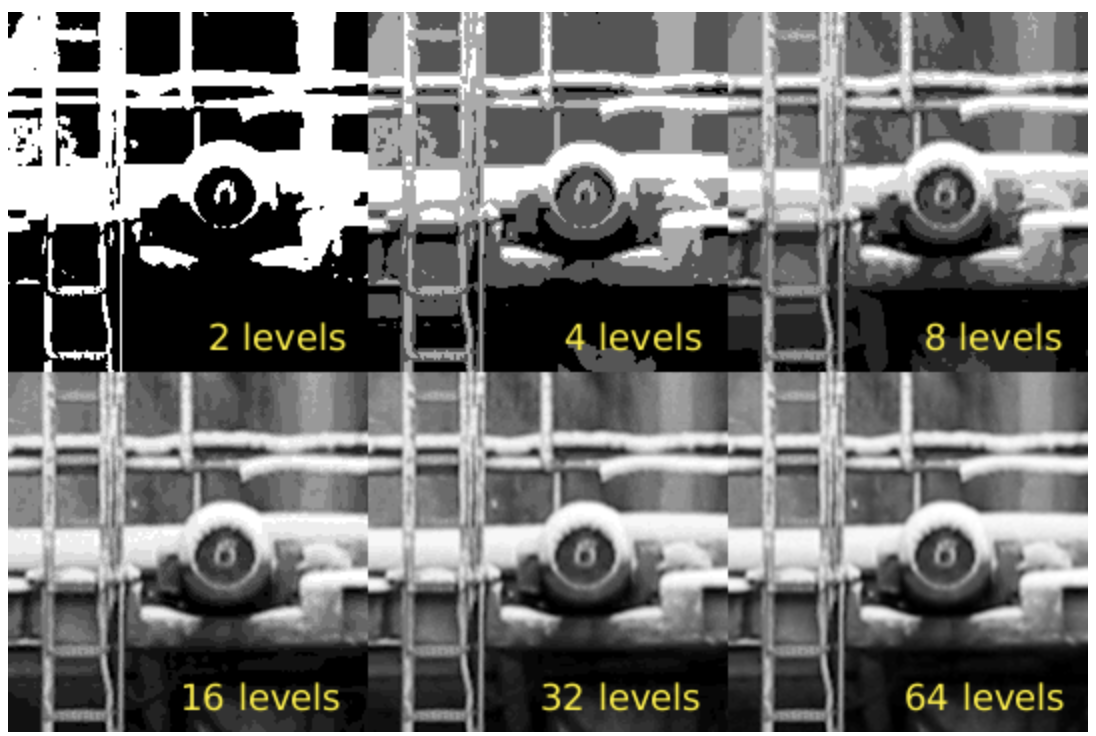
\includegraphics[scale=0.5]{image6.png}

    Рис. 6. Глибина зразка
\end{figure}

На рисунку 6 однакова ширина зображеннь.
Змінюється тільки глибина зразка.
Зауважте, що області з високою частотою (деталізовані області) мають добрий вигляд, ніж області з низькою частотою.

\section{8 біт}\label{sec:bit_eight}
Типовим форматом вибірки є 8-бітові цілі числа, 8-бітові цілі числа можуть представляти лише 256 дискретних значень (\(2^{8} = 256\)), таким чином рівні яскравості квантуються на ці рівні.

\section{12 біт}\label{sec:bit_twelve}
Для зображень із високим динамічним діапазоном (зображення з деталізацією як у тіні, так і у світлих місцях) 8-бітне 256 дискретних значень не забезпечує достатньої точності для збереження точного зображення.
Деякі цифрові камери внутрішньо працюють з більш ніж 8-бітними зразками, камери вищого класу також надають RAW-зображення, які часто мають 12 біт (\(2^{12} = 4096\)).

\section{16 біт}\label{sec:bit_sixteen}
Формати зображень PNG і TIF підтримують 16-бітні зразки, багато програм обробки зображень та маніпуляцій виконують свої операції в 16-бітному режимі, працюючи над 8-бітними зображеннями, щоб уникнути втрати якості при обробці.

\section{Плаваюча крапка (Floating point)}\label{sec:floating_point}
Деякі формати зображень, що використовуються в дослідженнях та у кіноіндустрії, зберігають значення з плаваючою комою.
Як "звичайні" 32-бітові значення з плаваючою комою, так і спеціальний формат, що називається \textbf{половина(half)}, який використовує 16 біт / зразок.
Зображення з плаваючою комою корисний як робочий формат, оскільки квантування та обчислювальні помилки зводяться до мінімуму до остаточного відтворення.

Представлення з плаваючою точкою часто включає HDR, \textbf{високий динамічний діапазон}.
Зображення з високим динамічним діапазоном - це зображення, що включають значення вибірки, які біліші від білого (вищі значення, ніж 255 для звичайного 8-бітного зображення).
HDR дозволяє представляти світло сцени з більшим ступенем точності, ніж зображення LDR із \textbf{низьким динамічним діапазоном}.

